\documentclass[12pt, centerh1]{article}
\textwidth=165mm \headheight=0mm \headsep=10mm \topmargin=-10mm
\textheight=230mm %\footskip=1.5cm
\oddsidemargin=0mm
%\documentclass[12pt,letterpaper]{article}
%\usepackage[margin=1in]{geometry}
\RequirePackage[colorlinks,citecolor=blue,urlcolor=blue]{hyperref}
\usepackage{amsmath, amssymb,natbib}
%\usepackage[mathscr]{euscript}
%\usepackage{mathrsfs}
\usepackage{graphicx,bm}
\usepackage{color}
\usepackage{subcaption}
\usepackage{subcaption}
\usepackage[table]{xcolor}
\usepackage{longtable}
\usepackage{amsthm}
\usepackage[mathscr]{euscript}
\usepackage{relsize}
\usepackage{amsmath,tabularx}
\newcolumntype{P}[1]{>{\centering\arraybackslash}p{#1}}
\usepackage{rotating}
\usepackage{eurosym}
\usepackage{colonequals}
\usepackage{bbm}
\usepackage{lscape}
\usepackage{natbib}

%%% make comments using the following setup %%
% type \your name {comment}, 
% e.g. \sophie{i love lyme disease}
\newcommand{\bruce}[1]{{\textcolor{blue}{$\langle$BC: #1$\rangle$}}}
\newcommand{\sophie}[1]{{\textcolor{purple}{$\langle$SS: #1$\rangle$}}}
\newcommand{\lauren}[1]{{\textcolor{cyan}{$\langle$LF: #1$\rangle$}}}
\newcommand{\geneva}[1]{{\textcolor{red}{$\langle$GL: #1$\rangle$}}}
\newcommand{\thanesh}[1]{{\textcolor{yellow}{$\langle$TR: #1$\rangle$}}}

\title{We care about acaricide $<3$}

%%% put in alphabetical order
\author{\qquad name$^{1,3}$ \qquad\  name$^{1}$ \qquad\  name$^{1,3}$ \\  name$^{2}$ \quad\ Sophie Stelmach$^{1}$}

\date{{\small $^1$ Department of Mathematics \& Statistics, McMaster University, Ontario, Canada.\\[-6pt]
$^2$ add your institution\\[-6pt]
$^3$ \\[-6pt]
}
}
\linespread{1.5}
\pdfminorversion=4

\begin{document}

% makes title
\maketitle



\section{Introduction}
Lyme disease is a highly emerging vector-borne disease in North America, which is caused by the bacterium \textit{Borrelia} and transmitted via infected bites of black-legged ticks (\textit{Ixodes}) \citep{govcan}. The risk of disease is further propagated by the changes in migratory patterns northward of these ticks by climate change.
sup bro yo
\subsection{Tick-host relationships}
\textbf{\textit{Borrelia}}, particularly B. burgdorferi sensu lato

\textbf{Black-legged tick}
I. scapularis is the primary cause of LD in Eastern North America. I. scapularis is also a vector for many types of pathogens such as Borrelia mayonni, Powassan virus and Anaplasma phaocytophilum \citep{paulson2023multiomics}. This shows that the black-legged tick can also increase the risk for polymicrobial infections besides just Lyme disease. Throughout the tick's life cycle, it encounters multiple hosts (Fig.1). When the eggs hatch, the larvae develop by feeding small mammals and birds. Since the ticks are naive when hatching, they get infected with the borrelia bacteria at this feeding stage, as small mammals and birds are carriers of this bacteria. As the larvae develop into nymphs, they seek new hosts. They can feed on rodents, birds, humans, and other small mammals at this stage. So, infected ticks can potentially feed on humans (terminal hosts) and infect them with B. burgdorferi sensu lato, which can lead to Lyme disease. Small mammals such as dogs and cats are incidental hosts who can also get bitten by infected nymph and potentially carry the ticks into households. Once nymphs develop into adult ticks, they feed, mate and lay eggs on only deer. Deer are an essential host for ticks to breed and propagate. Infected ticks pose the highest risk to humans during the larval and nymph stages as that is where the ticks first encounter the bacteria and can transmit it to humans or incidental hosts around humans. 

\subsection{Biology of Lyme disease}

\textbf{Lyme disease}
Lyme disease clinical manifestation can be divided into three stages; early localization, early dissemination and late persistence. 

\textbf{Lyme disease in Canada}
A study in eastern and southern Ontario, Canada found \textit{Borrelia} sp in approximately 70 percent of ticks with a relative abundance of 0.01 percent \citep{clow2018microbiota}. Concentration of adult \textit{I. scapularis} carrying endosymbiotic and pathogenic microorganisms in Southeastern Ontario \citep{paulson2023multiomics}. 


\subsection{Intervention}

In this study, a mathematical model was developed to evaluate the efficacy of acaricides as a Lyme disease intervention during the tick larval growth stage in Ontario, Canada. The potential for acaricides as an intervention has not been widely researched as of yet, and could prove to be useful as a way to control Lyme disease by killing ticks that feed on rodents. 

A study by \citet{dolan2004control} evaluated the efficacy of Fipronil, a rodent-targeted acaricide that is placed in bait boxes that rodents visit. Bait boxes such as the ones used in the study by \citet{dolan2004control} are commercially available, and the authors found that the lowest conentration of Fipronil required to kill tick nymps was 20 $\mu l$. To maintain a regular rate of visiting rodents, the box baits were placed ~10m apart from each other along a rodent path, and was rebaited and replenished with Fipronil every four weeks. In total, \citet{dolan2004control} report a 89\% reduction in the number of ticks per mouse, and a 53\% decrease in infection rate of ticks present on mice. After their 3 year experiment, only 33\% of adult ticks were infected with Lyme disease in sites with the bait boxes, compared to 47\% on sites without the bait boxes. The other advantage to these bait boxes is that many different tick hosts can visit a box and be treated with the acaricide and that there has been minimal environmental impact detected \citep{dolan2004control}. 

It is clear that there is a potential for using bait boxes with acaricide treatment as an intervention for preventing Lyme disease at the host level. In this paper, we will evaluate the effect of rodents visiting bait boxes and how the tick populations respond to the intervention.



\begin{figure}[h]
    \centering
    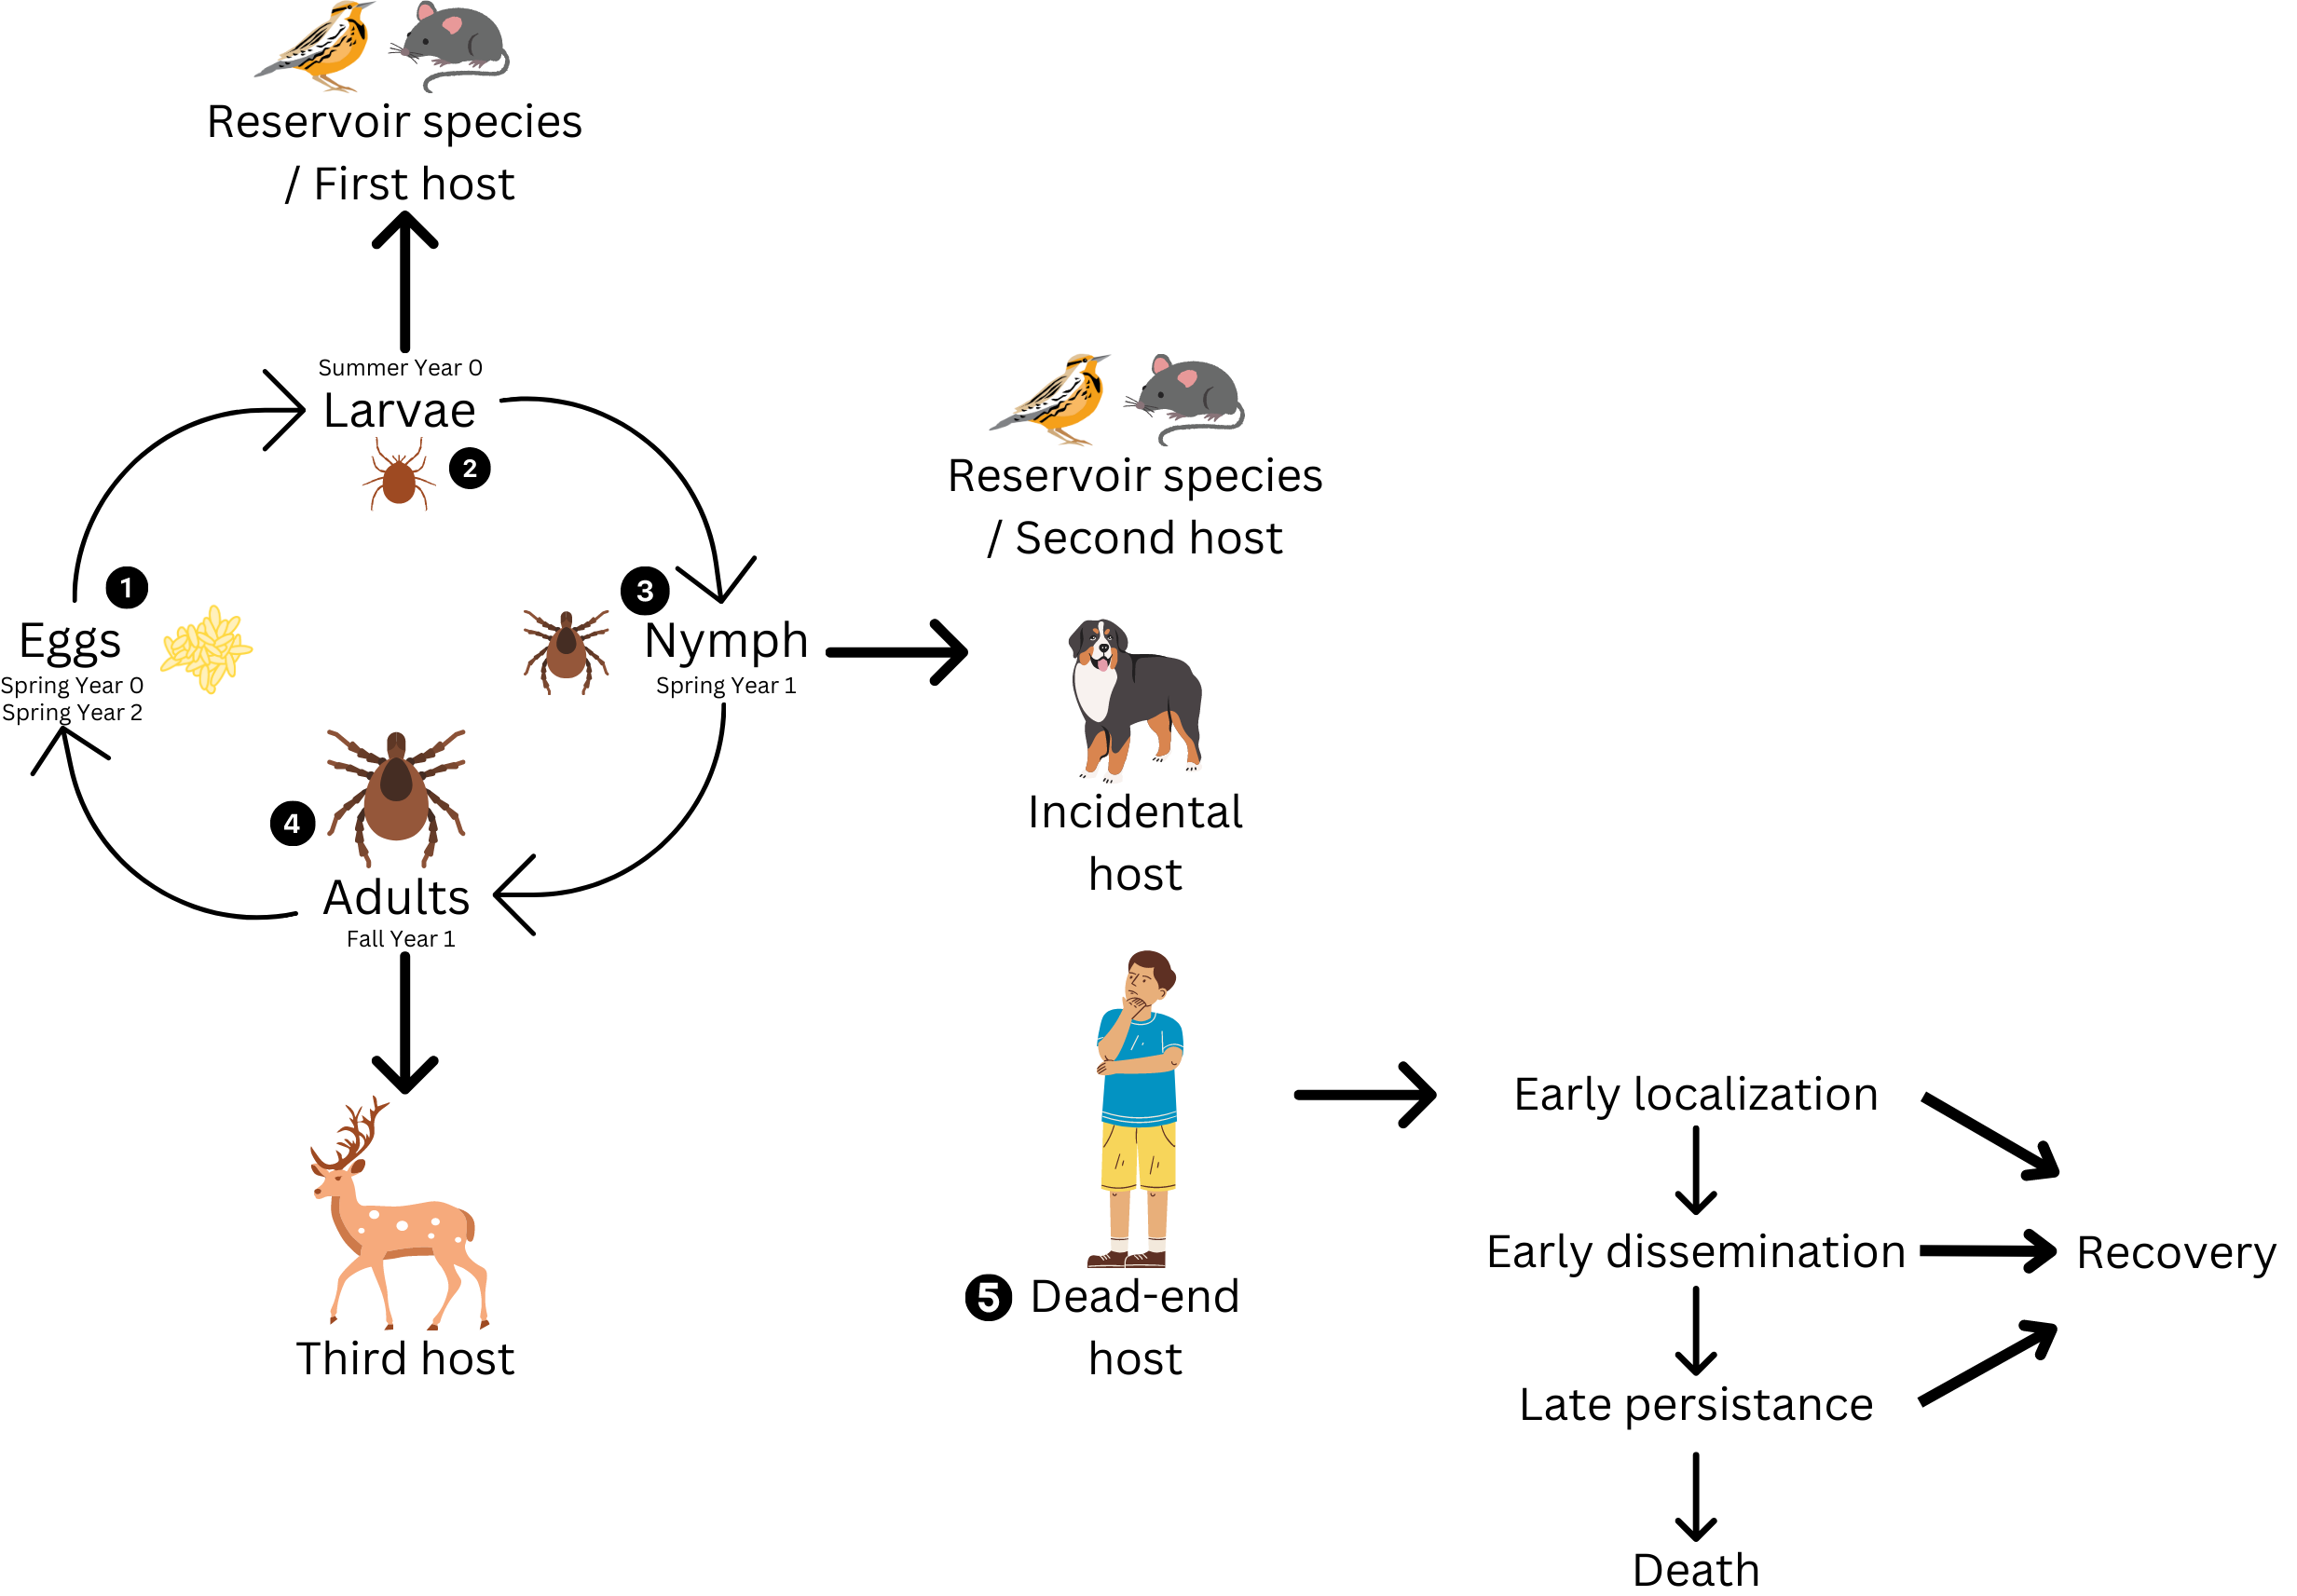
\includegraphics[scale = 0.15]{figures/Tick life cycle and progression of lyme disease.png}
    \caption{Diagram of tick life cycle and host bias.}
    \label{fig:lifecycle}
\end{figure}

\section{Methods}

\subsection{Proposed model}
The model proposed by \citet{lou2014tick} describes the tick life cycle and disease transmission between the tick and its hosts. The model features compartments that represent the various stages of the tick life cycle, including healthy ticks and infected ticks. We will base our analysis on this model, adding an intervention to prevent Lyme disease spread.

Ticks feed on their hosts in the larval, nymph, and adult stages of the life cycle, but primarily pose a risk to humans in the nymphal and adult phases. During the larval and nymphal stages, ticks will feel on small rodents, at which point they risk acquiring Lyme disease-causing bacteria \sophie{cite}. Larvae, nymphs and adults feed on their hosts at different rates, which is reflected in our model. 

This basic system, modelling a generic tick population along with tick and rodent infection rates, served as a basis for later outlined intervention method.

(system of diff equations)

This model, referring to values and parameters listed in \citet{lou2014tick}, takes into account the birth and death rates of ticks along with the rates at which they feed on feed on rodents in their respective stages of life. In this basic model, the total rodent population was treated as a constant value, and only the infectious rodents were incorporated.

\subsection{Rodent bait intervention}

to do: add new parameters to table (maybe a separate table?), make a table with our compartments and definitions, explain assumptions

\geneva{for now let's say S = susceptible, I = infected, P = poisonous}
\sophie{s could stand for seeking? as in seeking bait?}

Let's suppose $\theta$ is the death rate of ticks as a result of feeding on a rodent who has been treated with acaricide. For now we can assume this is 100\%?

Tick classes:
\begin{align}
    \frac{dL(t)}{dt} &= \left(b \,F_A - \frac{1}{K} A(t)\right)A(t) - (F_L + \mu_L) \,L(t) \\
    \frac{dN_S(t)}{dt} &= F_L\frac{R_S(t)}{R_S(t) + R_I(t) + R_P(t)}\,L(t) + (1-\beta_L)\,F_L \,L(t) \frac{R_I(t)}{R_S(t) + R_I(t) + R_P(t)} - (F_N + \mu_N) \,N_S(t) \\
    \frac{dN_I(t)}{dt} &= \beta_L F_L \,L(t) \frac{R_I(t)}{R_S(t) + R_I(t) + R_P(t)} - (F_N + \mu_N) \,N_I(t) \\
    \frac{dA_S(t)}{dt} &= F_N\frac{R_S(t)}{R_S(t) + R_I(t) + R_P(t)}\,N_S(t) - \mu_A \,A_S(t) \\
    \frac{dA_I(t)}{dt} &= F_N\left(1-\frac{R_P(t)}{R_S(t) + R_I(t) + R_P(t)}\right)\,N_I(t) + \beta_N \,F_N \,N_S(t) \, \frac{R_I(t)}{R_S(t) + R_I(t) + R_P(t)} - \mu_A \,A_I(t)
\end{align}

Rodent classes: \geneva{fix me later}
\begin{align}
    % \frac{dR_S(t)}{dt} &= -\beta_R F_N \,\frac{R_S(t)}{R_S(t) + R_I(t) + R_P(t)} \,N_I - (\nu + \mu_R) R_S(t) \\
    \frac{dR_S(t)}{dt} &= -\beta_R \, \sigma \,R_S(t) \frac{N_I(t)}{R_S(t) + R_I(t) + R_P(t)} - (\nu + \mu_R) R_S(t) \\
    % \frac{dR_I(t)}{dt} &= \beta_R F_N \,\frac{R_S(t)}{R_S(t) + R_I(t) + R_P(t)} \,N_I(t) - (\nu + \mu_R) R_I(t) \\
    \frac{dR_I(t)}{dt} &= \beta_R \,\sigma \,R_S(t) \frac{N_I(t)}{R_S(t) + R_I(t) + R_P(t)} - (\nu + \mu_R) R_I(t) \\
    \frac{dR_P(t)}{dt} &= \nu (R_S(t) + R_I(t)) - \mu_R R_P(t)
\end{align}

\subsection{Model assumptions}
- assumptions
- dynamics?

Similarly to \citet{lou2014tick}, we assume that adult ticks feed only on deer, and that larvae and nymph ticks feed on rodents. We will assume that these are the only tick hosts in the environment.

Furthermore, in the intervention model, we assume that there are only three compartments for rodents: susceptible/seeking, infectious, and poisonous. Susceptible rodents can become infectious or poisonous, and infectious rodents can become poisonous, however the opposite is not true. This is because once a rodent is poisonous, they cannot transmit disease to ticks because we assume all ticks feeding on poisonous rodents will die. Thus, the poison is said to have 100\% efficacy and no waning. Infectious rodents will remain infectious until they take the bait and become poisonous. All rodents die with the same mortality rate.

\geneva{Extended model assumptions: 100\% efficacy and no waning immunity/half-life, infected rodents stay infected forever unless they take the bait (``neutralise" the infection)}
\begin{center}
\begin{table}[h!]
\footnotesize
\noindent\makebox[\textwidth]{
 \begin{tabular}{||l l||} 
 \hline
 Parameter & Description \\ [0.5ex] 
 \hline\hline
 $R$ & Total number of rodents\\ 
 $D$ & Total number of the deer\\
 $F_L$ & Rate at which larval ticks attach on rodents. This is a function of R\\
 $F_N$ & Rate at which nymphal ticks bite rodents. This is a function of R\\ 
 $F_A$ & Rate at which adult ticks attack deer. This is a function of D\\
 $b$ & Larvae hatching per adult tick–deer interaction in the absence
of tick self-regulation\\
 $1/K$ & Scale of self-regulation in tick reproduction\\
 $\mu_L$ & Death rate for larval ticks\\
 $\mu_N$ & Death rate for nymphal ticks\\ 
 $\mu_R$ & Death rate for rodents\\
 $\mu_A$ & Death rate for adult ticks\\
 $\beta_L$ & Transmission coefficient of spirochete infection to rodents\\
 $\beta_N$ & Transmission coefficient of spirochete infection to larval ticks\\
 $\beta_A$ & Transmission coefficient of spirochete infection to nymphal ticks\\[1ex] 
 \hline
 \end{tabular}
 }
\end{table}
\end{center}


\section{Results}



\section{Discussion}

- we only looked at rodents as hosts of lyme disease, but there are many other small animals eg chipmunks that act as hosts. they could also be treated with acaricide 
- the boxes dont require a lot of maintenance, only every 3-4 weeks do the boxes need to be replenished with bait and treatment
- need to be placed in early may in areas where hosts reside, in quantities relative to the density of hosts in that region


\subsection{Model Implications}

\subsection{Effect on Policy Decisions}

\subsection{Future Studies}


\section{Conclusion}



\newpage
\bibliographystyle{chicago} %idk what style we want to do
\bibliography{bib}
\end{document}
